\chapter*{Appendix: Swarmalators on an ER Network}
We now explore how the active phase wave state ($K = -0.6$, $J = 0.9$) behaves on an Erdős-Rényi (ER) network as the connection probability $p$ increases.

\section{Order Parameters}
A useful way to assess the system's state is through three order parameters \cite{O_Keeffe_2017}, independent of the network topology:
\begin{itemize}
    \item \( r \) measures the degree of phase synchronization, ranging from 0 (desynchronized) to 1 (fully synchronized), as introduced in the Kuramoto model \cite{Acebron_2005}:
    \begin{equation}
        r = \left| \frac{1}{N} \sum_{j=1}^{N} e^{i \theta_j} \right|
        \label{equation::r}
    \end{equation}
    \item \( S \) quantifies the correlation between phases \( \theta_j \) and spatial angles \( \phi_j \):
    \begin{equation}
        S = \max \left\{  \left| \frac{1}{N} \sum_{j=1}^{N} e^{i (\phi_j+\theta_j)} \right|, \left| \frac{1}{N} \sum_{j=1}^{N} e^{i (\phi_j-\theta_j)} \right| \right\}
        \label{equation::S}
    \end{equation}
    \item \( U \) measures the fraction of swarmalators that complete at least one full cycle in both space and phase:
    \begin{equation}
        U = \frac{N_{rot}}{N}
        \label{equation::U}
    \end{equation}
\end{itemize}
\( S \) is positive in both splintered and active phase wave states, while \( U \) is non-zero only in the active phase wave.

\newpage
\section{ER Network}
Using tools from the third laboratory, we implemented functions to compute the order parameters for each simulation. After reaching the steady state ($t_f = 300$), we computed \( r \), \( S \) (discarding the transient dynamics), and \( U \). Each value of $p$ was averaged over five different realizations of the system to obtain means and standard deviations.

%if time improve to ten

The results for $S$ and $U$ are shown below.

\begin{figure}[h]
    \centering
    \begin{minipage}[c]{0.8\textwidth}
        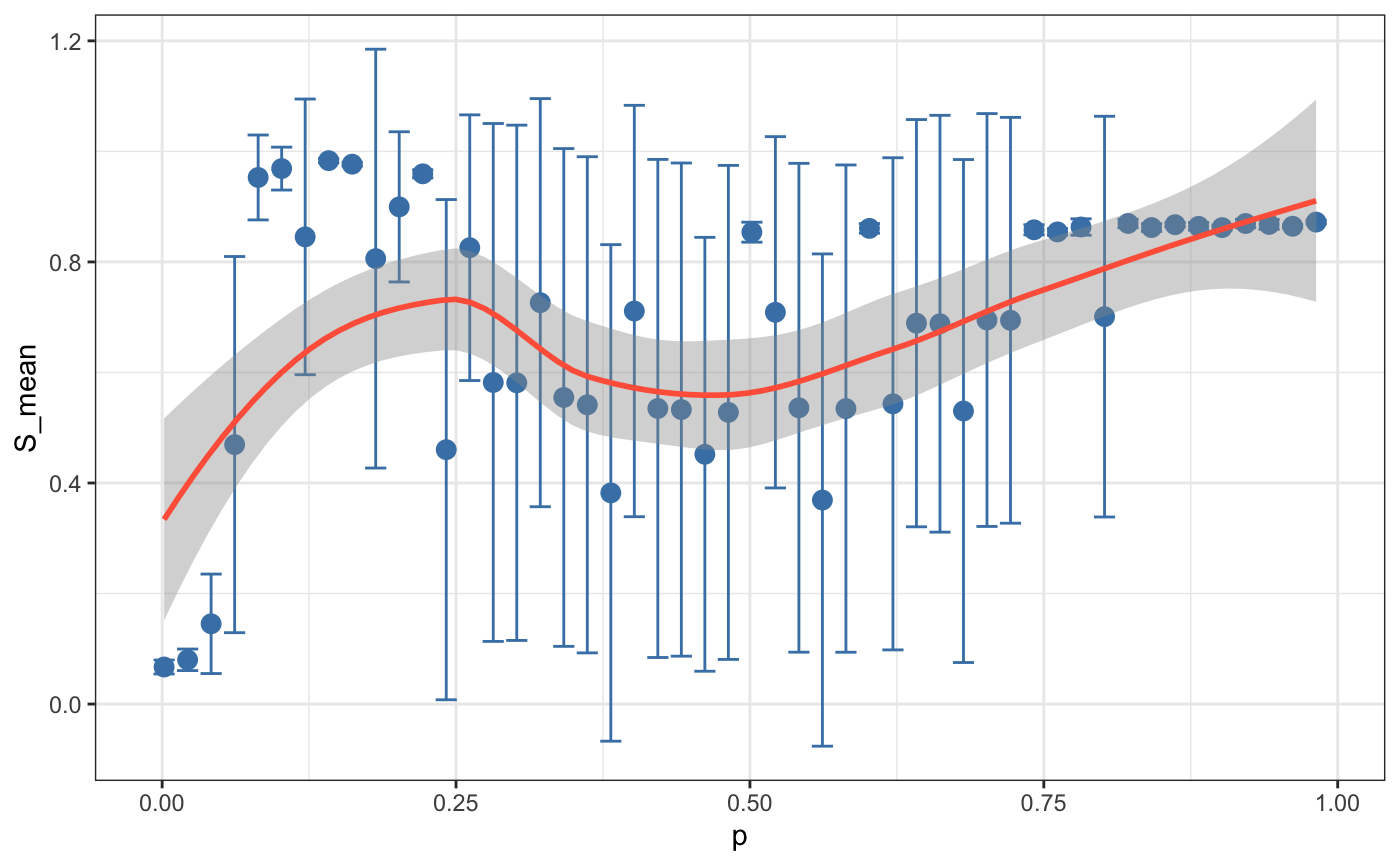
\includegraphics[width=\textwidth]{images/task20-appendix/S_K=-0.6,J=0.9.png}
    \end{minipage}
    \label{fig:S}
\end{figure}

\begin{figure}[h]
    \centering
    \begin{minipage}[c]{0.8\textwidth}
        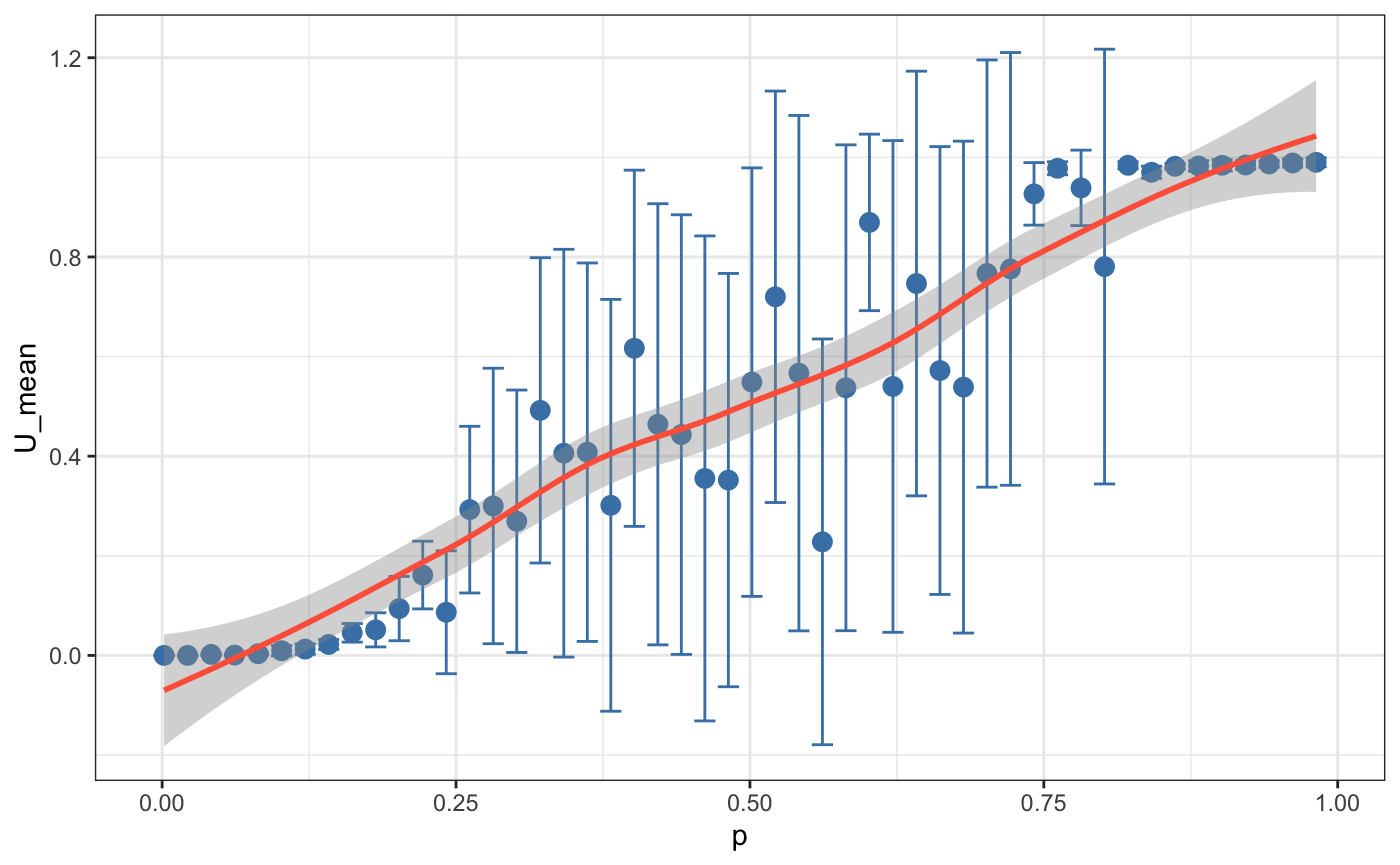
\includegraphics[width=\textwidth]{images/task20-appendix/U_K=-0.6,J=0.9.png}
    \end{minipage}
    \label{fig:U}
\end{figure}

Due to the significant errors observed for intermediate values of $p$ (likely a consequence of the limited simulation time, which could be greatly improved), only limited conclusions can be drawn regarding the functional forms of the order parameters. However, for both $S$ and $U$, we can distinguish a region at low $p$, where the value is zero, and regions at higher $p$ values, closer to 1, where the parameters seem to approach asymptotic values. 

It is possible that, as connectivity increases, more swarmalators interact, leading to greater spatial-phase rotation and synchronization. For $S$ this could also be related to the emergence of the giant connected component (GCC).



